\begin{figure}[H]
    \centering
    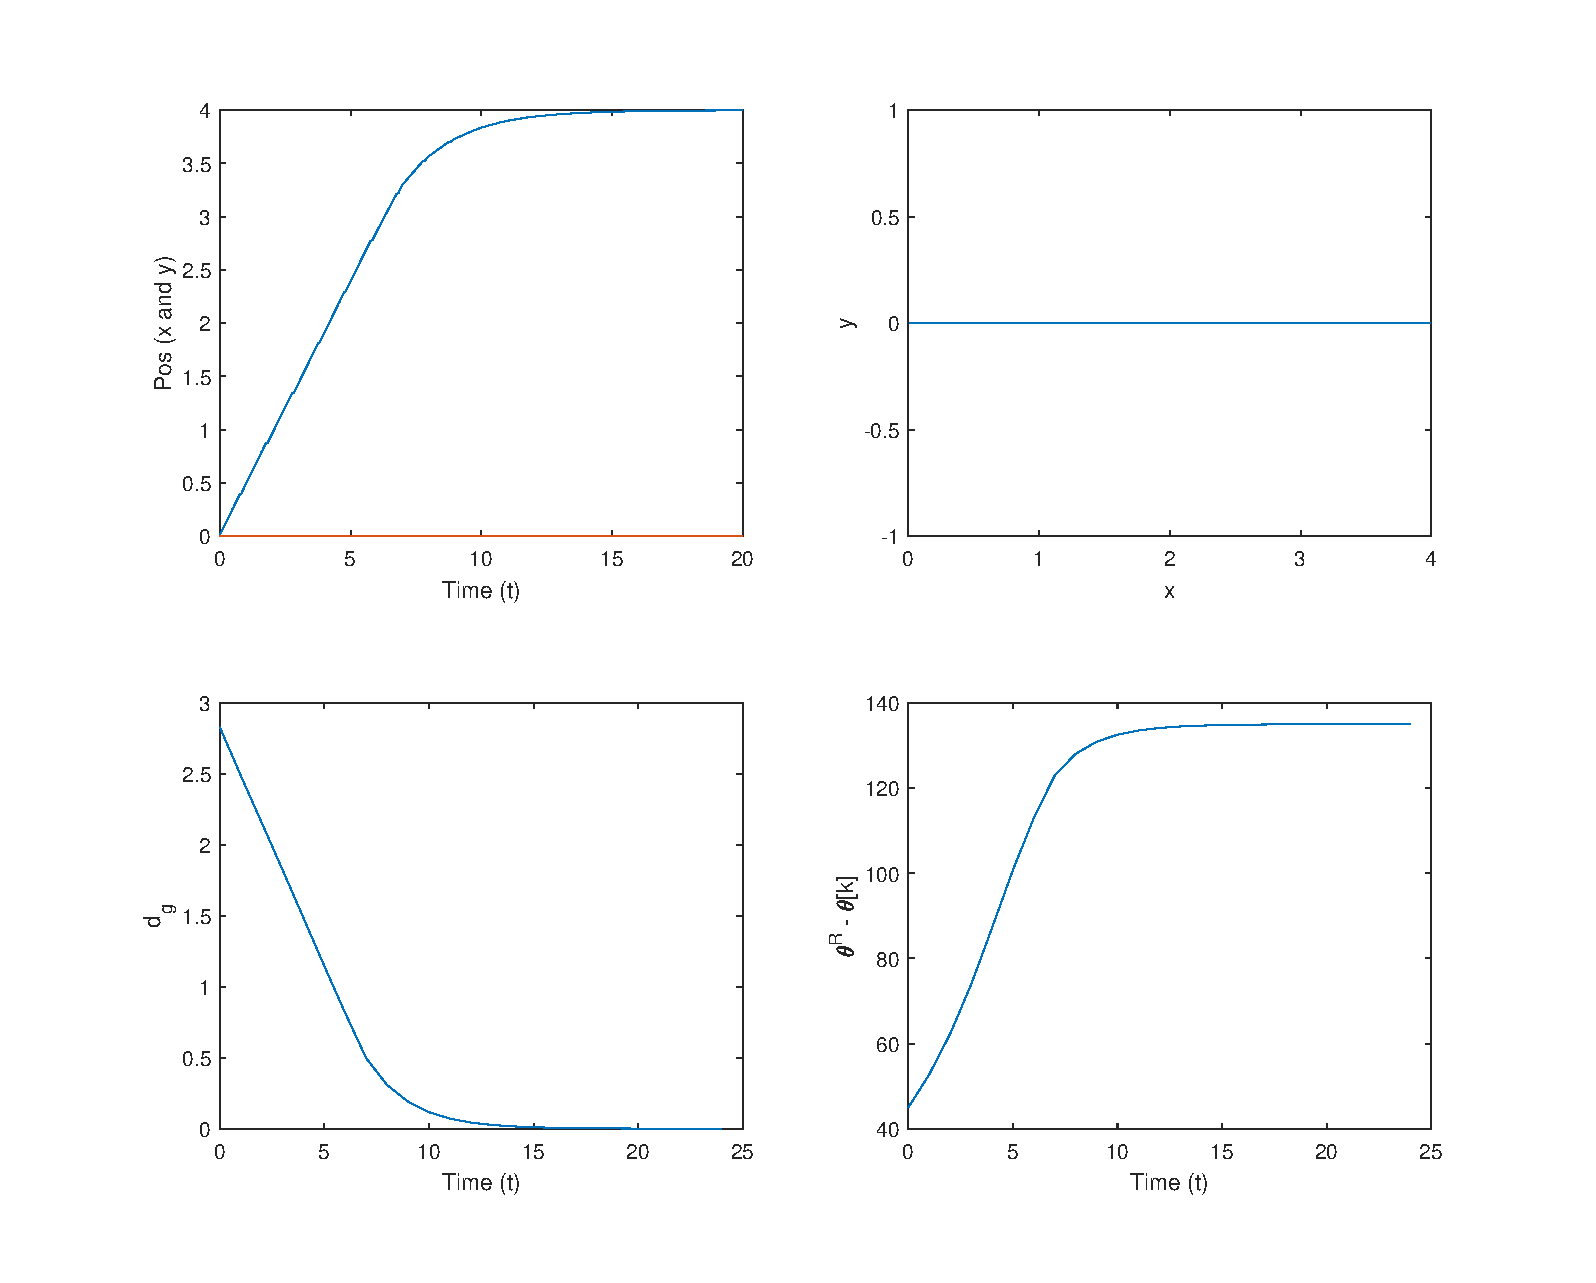
\includegraphics[width=\textwidth]{figs/perf-dg.eps}
    \caption{Simulation of the $d_g$  controller going from $(0, 0)$ to $(2, 2)$ with $K_\omega= \frac{180}{R \pi}.$}\label{fig:perf-dg}
\end{figure}

The controller drives the robot to a position orthogonal to the goal position on the line between $(x_0, y_0)$ and $(x_g, y_g)$. Since $K_\omega$ is set to give a dead beat controller the robot should get close to to the goal position if it starts in the direction of the goal. Otherwise it will not reach the goal position.